\documentclass{standalone}
\usepackage{tikz}
\usetikzlibrary{patterns, positioning}


\begin{document}
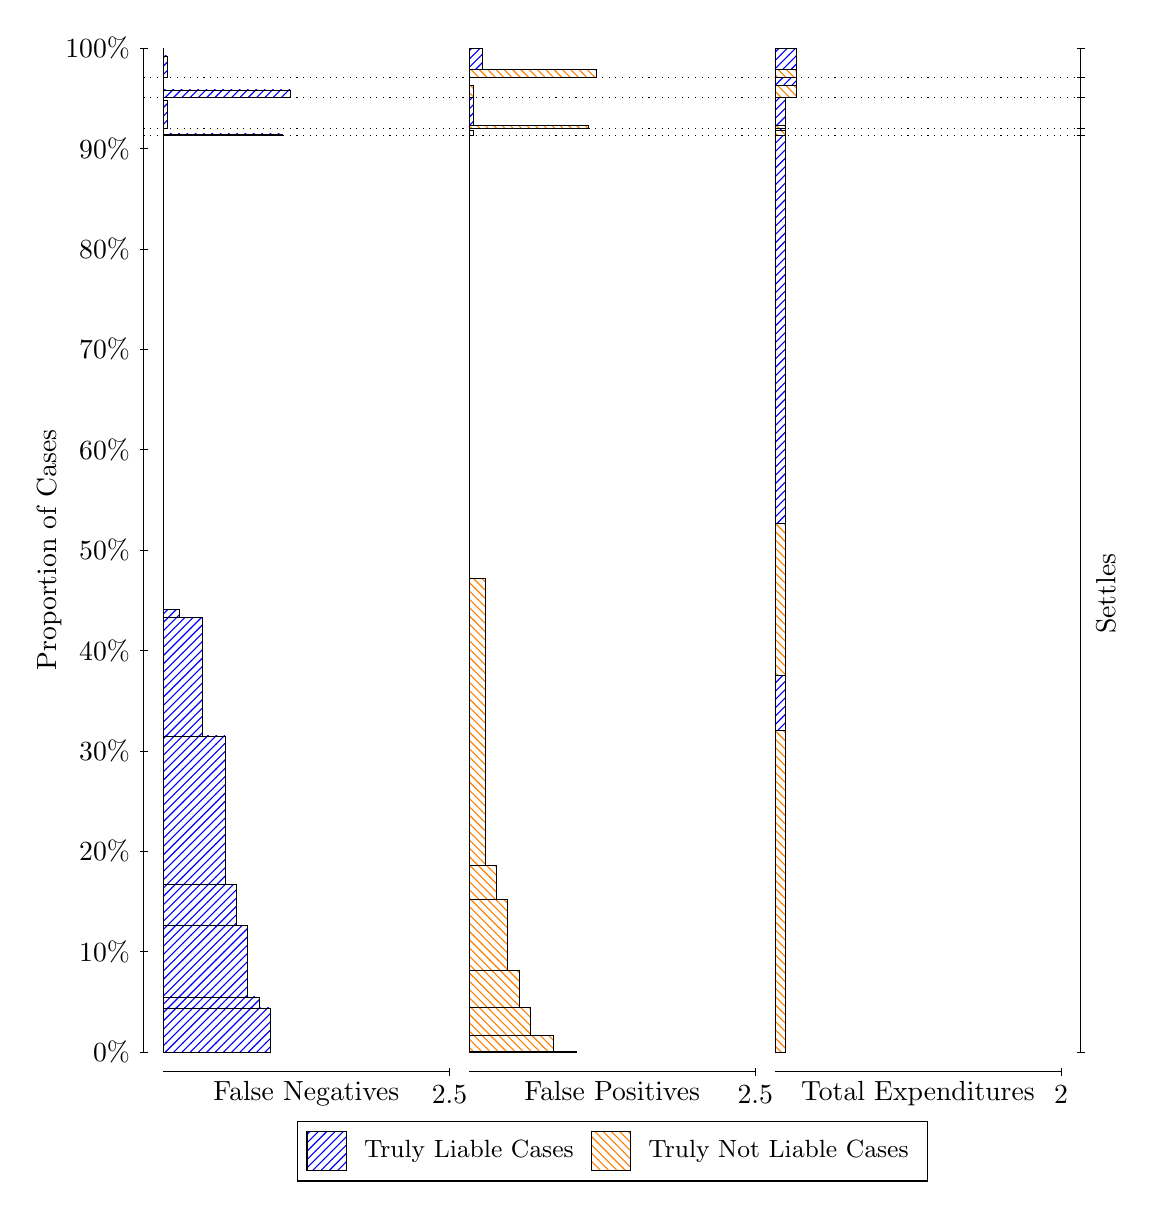
\begin{tikzpicture}
\draw[black, very thin] (1.5,1.75) -- (1.5,14.5);
\node[rotate=90, text=black, anchor=center] at (0.3, 8.125) {Proportion of Cases};
\draw[black, very thin] (1.45,1.75) -- (1.55,1.75);
\node[text=black, anchor=east] at (1.45, 1.75) {0\%};
\draw[black, very thin] (1.45,3.025) -- (1.55,3.025);
\node[text=black, anchor=east] at (1.45, 3.025) {10\%};
\draw[black, very thin] (1.45,4.3) -- (1.55,4.3);
\node[text=black, anchor=east] at (1.45, 4.3) {20\%};
\draw[black, very thin] (1.45,5.575) -- (1.55,5.575);
\node[text=black, anchor=east] at (1.45, 5.575) {30\%};
\draw[black, very thin] (1.45,6.85) -- (1.55,6.85);
\node[text=black, anchor=east] at (1.45, 6.85) {40\%};
\draw[black, very thin] (1.45,8.125) -- (1.55,8.125);
\node[text=black, anchor=east] at (1.45, 8.125) {50\%};
\draw[black, very thin] (1.45,9.4) -- (1.55,9.4);
\node[text=black, anchor=east] at (1.45, 9.4) {60\%};
\draw[black, very thin] (1.45,10.675) -- (1.55,10.675);
\node[text=black, anchor=east] at (1.45, 10.675) {70\%};
\draw[black, very thin] (1.45,11.95) -- (1.55,11.95);
\node[text=black, anchor=east] at (1.45, 11.95) {80\%};
\draw[black, very thin] (1.45,13.225) -- (1.55,13.225);
\node[text=black, anchor=east] at (1.45, 13.225) {90\%};
\draw[black, very thin] (1.45,14.5) -- (1.55,14.5);
\node[text=black, anchor=east] at (1.45, 14.5) {100\%};

\draw[black, very thin] (13.4,1.75) -- (13.4,14.5);
\draw[black, very thin] (13.35,1.75) -- (13.45,1.75);
\node[anchor=west] at (13.35, 1.75) {};
\draw[black, very thin] (13.35,13.389) -- (13.45,13.389);
\node[anchor=west] at (13.35, 13.389) {};
\draw[black, very thin] (13.35,13.479) -- (13.45,13.479);
\node[anchor=west] at (13.35, 13.479) {};
\draw[black, very thin] (13.35,13.869) -- (13.45,13.869);
\node[anchor=west] at (13.35, 13.869) {};
\draw[black, very thin] (13.35,14.124) -- (13.45,14.124);
\node[anchor=west] at (13.35, 14.124) {};
\draw[black, very thin] (13.35,14.5) -- (13.45,14.5);
\node[anchor=west] at (13.35, 14.5) {};

\draw[black, very thin, pattern color=blue, pattern=north east lines] (1.75,1.75) rectangle (3.1125,2.309);
\draw[black, very thin, pattern color=blue, pattern=north east lines] (1.75,2.309) rectangle (2.9672,2.4504);
\draw[black, very thin, pattern color=blue, pattern=north east lines] (1.75,2.4504) rectangle (2.8218,3.3613);
\draw[black, very thin, pattern color=blue, pattern=north east lines] (1.75,3.3613) rectangle (2.6765,3.882);
\draw[black, very thin, pattern color=blue, pattern=north east lines] (1.75,3.882) rectangle (2.5312,5.763);
\draw[black, very thin, pattern color=blue, pattern=north east lines] (1.75,5.763) rectangle (2.2405,7.2664);
\draw[black, very thin, pattern color=blue, pattern=north east lines] (1.75,7.2664) rectangle (1.9498,7.3719);
\draw[black, very thin, pattern color=orange, pattern=north west lines] (1.75,7.3719) rectangle (1.75,13.389);
\draw[black, very thin, pattern color=blue, pattern=north east lines] (1.75,13.389) rectangle (3.2578,13.41);
\draw[black, very thin, pattern color=orange, pattern=north west lines] (1.75,13.41) rectangle (1.75,13.479);
\draw[black, very thin, pattern color=blue, pattern=north east lines] (1.75,13.479) rectangle (1.8045,13.835);
\draw[black, very thin, pattern color=orange, pattern=north west lines] (1.75,13.835) rectangle (1.75,13.869);
\draw[black, very thin, pattern color=blue, pattern=north east lines] (1.75,13.869) rectangle (3.3668,13.969);
\draw[black, very thin, pattern color=orange, pattern=north west lines] (1.75,13.969) rectangle (1.75,14.124);
\draw[black, very thin, pattern color=blue, pattern=north east lines] (1.75,14.124) rectangle (1.8045,14.4);
\draw[black, very thin, pattern color=orange, pattern=north west lines] (1.75,14.4) rectangle (1.75,14.5);
\draw[black, very thin, pattern color=orange, pattern=north west lines] (5.6333,1.75) rectangle (6.9958,1.7574);
\draw[black, very thin, pattern color=orange, pattern=north west lines] (5.6333,1.7574) rectangle (6.7052,1.9616);
\draw[black, very thin, pattern color=orange, pattern=north west lines] (5.6333,1.9616) rectangle (6.4145,2.316);
\draw[black, very thin, pattern color=orange, pattern=north west lines] (5.6333,2.316) rectangle (6.2692,2.7865);
\draw[black, very thin, pattern color=orange, pattern=north west lines] (5.6333,2.7865) rectangle (6.1238,3.6853);
\draw[black, very thin, pattern color=orange, pattern=north west lines] (5.6333,3.6853) rectangle (5.9785,4.1193);
\draw[black, very thin, pattern color=orange, pattern=north west lines] (5.6333,4.1193) rectangle (5.8332,7.7674);
\draw[black, very thin, pattern color=blue, pattern=north east lines] (5.6333,7.7674) rectangle (5.6333,13.389);
\draw[black, very thin, pattern color=orange, pattern=north west lines] (5.6333,13.389) rectangle (5.6878,13.458);
\draw[black, very thin, pattern color=blue, pattern=north east lines] (5.6333,13.458) rectangle (5.6333,13.479);
\draw[black, very thin, pattern color=orange, pattern=north west lines] (5.6333,13.479) rectangle (7.1412,13.513);
\draw[black, very thin, pattern color=blue, pattern=north east lines] (5.6333,13.513) rectangle (5.6878,13.869);
\draw[black, very thin, pattern color=orange, pattern=north west lines] (5.6333,13.869) rectangle (5.6878,14.025);
\draw[black, very thin, pattern color=blue, pattern=north east lines] (5.6333,14.025) rectangle (5.6333,14.124);
\draw[black, very thin, pattern color=orange, pattern=north west lines] (5.6333,14.124) rectangle (7.2502,14.224);
\draw[black, very thin, pattern color=blue, pattern=north east lines] (5.6333,14.224) rectangle (5.7968,14.5);
\draw[black, very thin, pattern color=orange, pattern=north west lines] (9.5167,1.75) rectangle (9.6529,5.8321);
\draw[black, very thin, pattern color=blue, pattern=north east lines] (9.5167,5.8321) rectangle (9.6529,6.5326);
\draw[black, very thin, pattern color=orange, pattern=north west lines] (9.5167,6.5326) rectangle (9.6529,8.4679);
\draw[black, very thin, pattern color=blue, pattern=north east lines] (9.5167,8.4679) rectangle (9.6529,13.389);
\draw[black, very thin, pattern color=orange, pattern=north west lines] (9.5167,13.389) rectangle (9.6529,13.458);
\draw[black, very thin, pattern color=blue, pattern=north east lines] (9.5167,13.458) rectangle (9.6529,13.479);
\draw[black, very thin, pattern color=orange, pattern=north west lines] (9.5167,13.479) rectangle (9.6529,13.513);
\draw[black, very thin, pattern color=blue, pattern=north east lines] (9.5167,13.513) rectangle (9.6529,13.869);
\draw[black, very thin, pattern color=orange, pattern=north west lines] (9.5167,13.869) rectangle (9.7892,14.025);
\draw[black, very thin, pattern color=blue, pattern=north east lines] (9.5167,14.025) rectangle (9.7892,14.124);
\draw[black, very thin, pattern color=orange, pattern=north west lines] (9.5167,14.124) rectangle (9.7892,14.224);
\draw[black, very thin, pattern color=blue, pattern=north east lines] (9.5167,14.224) rectangle (9.7892,14.5);
\draw[black, dotted] (1.5,13.389) -- (13.4,13.389);
\draw[black, dotted] (1.5,13.479) -- (13.4,13.479);
\draw[black, dotted] (1.5,13.869) -- (13.4,13.869);
\draw[black, dotted] (1.5,14.124) -- (13.4,14.124);
\draw[black, very thin] (1.75,1.5) -- (5.3833,1.5);
\node[text=black, anchor=north] at (3.5667, 1.5) {False Negatives};
\draw[black, very thin] (5.3833,1.45) -- (5.3833,1.55);
\node[text=black, anchor=north] at (5.3833, 1.45) {2.5};

\draw[black, very thin] (5.6333,1.5) -- (9.2667,1.5);
\node[text=black, anchor=north] at (7.45, 1.5) {False Positives};
\draw[black, very thin] (9.2667,1.45) -- (9.2667,1.55);
\node[text=black, anchor=north] at (9.2667, 1.45) {2.5};

\draw[black, very thin] (9.5167,1.5) -- (13.15,1.5);
\node[text=black, anchor=north] at (11.333, 1.5) {Total Expenditures};
\draw[black, very thin] (13.15,1.45) -- (13.15,1.55);
\node[text=black, anchor=north] at (13.15, 1.45) {2};

\node[text=black, centered, rotate=90] at (13.72, 7.5697) {Settles};





\draw (7.449999999999999,1.5) node[draw=none] (baseCoordinate) {};
\begin{scope}[align=center]
        \matrix[scale=0.5, draw=black, below=0.5cm of baseCoordinate, nodes={draw}, column sep=0.1cm]{
            \node[rectangle, draw, minimum width=0.5cm, minimum height=0.5cm, pattern color=blue, pattern=north east lines] {}; &
            \node[draw=none, font=\small, text=black] (B) {Truly Liable Cases}; &
            \node[rectangle, draw, minimum width=0.5cm, minimum height=0.5cm, pattern color=orange, pattern=north west lines] {}; &
            \node[draw=none, font=\small, text=black] (B) {Truly Not Liable Cases}; \\
            };
\end{scope}

\end{tikzpicture}
\end{document}